\documentclass[aspectratio=169,11pt]{beamer}

% ============================================================
% Theme (from your 11pt preamble)
% ============================================================
\usetheme{Madrid}
\usecolortheme{seahorse}
\setbeamertemplate{navigation symbols}{}

% ============================================================
% Encoding (pdfLaTeX-safe)
% ============================================================
\usepackage[utf8]{inputenc}
\usepackage[T1]{fontenc}
\usepackage{lmodern}

% ============================================================
% Packages (merge)
% ============================================================
\usepackage{amsmath}
\usepackage{xcolor}
\usepackage{listings}
\usepackage{tikz}

% ============================================================
% Listings style (use your 11pt preamble style)
% ============================================================
\lstset{
	basicstyle=\ttfamily\small,
	frame=single,
	breaklines=true,
	columns=fullflexible,
	keywordstyle=\color{blue},
	commentstyle=\color{gray},
	stringstyle=\color{red},
	showstringspaces=false
}

% ============================================================
% Title (keep your identity block)
% ============================================================
\title{Concurrency \& Distributed Systems}
\subtitle{Week 2 --- Day 1: Threads: Mental Model + Creation Patterns}
\author{Dr. Mohamad Aoude}
\institute{Lebanese University \\ Faculty of Engineering}
\date{\today}

% ============================================================
\begin{document}
	
	% ------------------------------------------------
	\begin{frame}
		\titlepage
	\end{frame}
	
	% ------------------------------------------------
	\begin{frame}{Disruptive Question}
		\begin{block}{Think}
			If I create two threads in Java... \\
			\textbf{Do they really run at the same time?}
		\end{block}
		
		\vspace{5mm}
		
		If I create 8 threads on a 4-core CPU... \\
		\textbf{What is actually happening?}
	\end{frame}
	
	% ------------------------------------------------
	\begin{frame}{Illusion vs Reality}
		\begin{center}
			\Huge
			Illusion \quad $\neq$ \quad Reality
		\end{center}
		
		\vspace{5mm}
		
		\begin{itemize}
			\item Concurrency is not magic
			\item The OS decides execution
			\item Order is not guaranteed
		\end{itemize}
	\end{frame}
	
	% ------------------------------------------------
	\begin{frame}{What Is a Process?}
		\begin{center}
			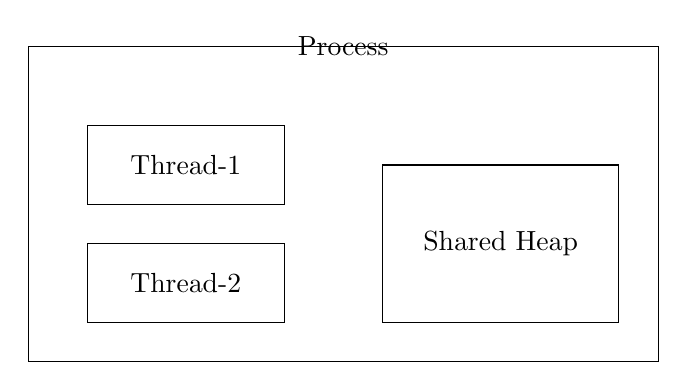
\begin{tikzpicture}
				\node[draw, minimum width=8cm, minimum height=4cm] (process) {};
				\node at (process.north) {Process};
				
				\node[draw, minimum width=2.5cm, minimum height=1cm] at (-2,0.5) {Thread-1};
				\node[draw, minimum width=2.5cm, minimum height=1cm] at (-2,-1) {Thread-2};
				\node[draw, minimum width=3cm, minimum height=2cm] at (2,-0.5) {Shared Heap};
			\end{tikzpicture}
		\end{center}
	\end{frame}
	
	% ------------------------------------------------
	\begin{frame}{Thread Memory Model}
		\begin{block}{Each Thread Has}
			\begin{itemize}
				\item Its own Stack
				\item Its own Program Counter
				\item Its own Local Variables
			\end{itemize}
		\end{block}
		
		\begin{block}{All Threads Share}
			\begin{itemize}
				\item Heap (Objects)
				\item Static Variables
				\item Files / Sockets
			\end{itemize}
		\end{block}
	\end{frame}
	
	% ------------------------------------------------
	\begin{frame}{Critical Precision}
		\begin{center}
			\Large
			Reference Location $\neq$ Object Location
		\end{center}
		
		\vspace{5mm}
		
		\begin{itemize}
			\item Local variable may be private
			\item Object it points to may be shared
			\item This is where race conditions begin
		\end{itemize}
	\end{frame}
	
	% ------------------------------------------------
	\begin{frame}{Who Schedules Threads?}
		\begin{block}{Important}
			JVM creates threads. \\
			\textbf{OS schedules them.}
		\end{block}
		
		\vspace{4mm}
		
		\begin{center}
			JVM $\neq$ CPU Scheduler
		\end{center}
		
		\vspace{4mm}
		
		Execution order is \textbf{nondeterministic}.
	\end{frame}
	
	% ------------------------------------------------
	\begin{frame}{Time Slicing (Reality)}
		\begin{center}
			\Huge
			T1 \quad T2 \quad T1 \quad T2 \quad T2 \quad T1
		\end{center}
		
		\vspace{5mm}
		
		Threads are:
		\begin{itemize}
			\item Preempted
			\item Interleaved
			\item Time-sliced
		\end{itemize}
	\end{frame}
	
	% ------------------------------------------------
	\begin{frame}[fragile]{Interrupt Discipline}
		\begin{block}{Never Swallow Interrupts}
		\end{block}
		
		\begin{lstlisting}
			catch (InterruptedException e) {
				Thread.currentThread().interrupt();
			}
		\end{lstlisting}
		
		\begin{itemize}
			\item Interrupt = cancellation signal
			\item Swallowing creates zombie threads
			\item Professional Java respects interruption
		\end{itemize}
	\end{frame}
	
	% ------------------------------------------------
	\begin{frame}[fragile]{Pattern 1 — Extending Thread}
		\begin{lstlisting}
			class MyThread extends Thread {
				public void run() {
					System.out.println(getName());
				}
			}
			
			MyThread t = new MyThread();
			t.start();
		\end{lstlisting}
		
		\begin{itemize}
			\item Task tightly coupled to Thread
			\item Single inheritance limitation
		\end{itemize}
	\end{frame}
	
	% ------------------------------------------------
	\begin{frame}[fragile]{Pattern 2 — Runnable (Preferred)}
		\begin{lstlisting}
			class MyTask implements Runnable {
				public void run() {
					System.out.println(
					Thread.currentThread().getName()
					);
				}
			}
			
			Thread t = new Thread(new MyTask());
			t.start();
		\end{lstlisting}
		
		\begin{center}
			\Large
			Task $\neq$ Thread
		\end{center}
	\end{frame}
	
	% ------------------------------------------------
	\begin{frame}[fragile]{Pattern 3 — Lambda}
		\begin{lstlisting}
			Thread t = new Thread(() -> {
				System.out.println(
				Thread.currentThread().getName()
				);
			}, "Lambda-Worker");
			
			t.start();
		\end{lstlisting}
		
		Runnable = Functional Interface
	\end{frame}
	
	% ------------------------------------------------
	\begin{frame}[fragile]{Critical Mistake: run() vs start()}
		\begin{lstlisting}
			Thread t = new Thread(() ->
			System.out.println(
			Thread.currentThread().getName()
			)
			);
			
			t.run();   // What happens?
		\end{lstlisting}
		
		\pause
		
		\begin{center}
			Prints: \textbf{main}
		\end{center}
	\end{frame}
	
	% ------------------------------------------------
	\begin{frame}[fragile]{Correct Way}
		\begin{lstlisting}
			t.start();
		\end{lstlisting}
		
		\begin{center}
			\Large
			run() = synchronous \\
			start() = asynchronous
		\end{center}
		
		\vspace{4mm}
		
		start() creates a new call stack.
	\end{frame}
	
	% ------------------------------------------------
	\begin{frame}[fragile]{Interleaving Demonstration}
		\begin{lstlisting}
			Thread t1 = new Thread(() -> {
				for (int i = 0; i < 5; i++)
				System.out.println("T1-" + i);
			});
			
			Thread t2 = new Thread(() -> {
				for (int i = 0; i < 5; i++)
				System.out.println("T2-" + i);
			});
			
			t1.start();
			t2.start();
		\end{lstlisting}
		
		Execution order is unpredictable.
	\end{frame}
	
	% ------------------------------------------------
	\begin{frame}[fragile]{Sleep Myth}
		\begin{lstlisting}
			Thread.sleep(1);
		\end{lstlisting}
		
		\begin{itemize}
			\item Sleep does NOT guarantee order
			\item Sleep does NOT enforce fairness
			\item Sleep does NOT release locks
		\end{itemize}
	\end{frame}
	
	% ------------------------------------------------
	\begin{frame}{Block 1 Summary}
		\begin{itemize}
			\item Thread = schedulable execution unit
			\item Stack = private
			\item Heap = shared
			\item OS schedules
			\item run() $\neq$ start()
			\item Order is not guaranteed
			\item Interleaving is normal
		\end{itemize}
		
		\vspace{5mm}
		
		\begin{center}
			\Large
			Today you lost control over time. \\
			Tomorrow you regain control over access.
		\end{center}
	\end{frame}
	
	% ------------------------------------------------
\end{document}
